\documentclass[11pt,]{article}
\usepackage[left=1in,top=1in,right=1in,bottom=1in]{geometry}
\newcommand*{\authorfont}{\fontfamily{phv}\selectfont}
\usepackage[]{mathpazo}


  \usepackage[T1]{fontenc}
  \usepackage[utf8]{inputenc}




\usepackage{abstract}
\renewcommand{\abstractname}{}    % clear the title
\renewcommand{\absnamepos}{empty} % originally center

\renewenvironment{abstract}
 {{%
    \setlength{\leftmargin}{0mm}
    \setlength{\rightmargin}{\leftmargin}%
  }%
  \relax}
 {\endlist}

\makeatletter
\def\@maketitle{%
  \newpage
%  \null
%  \vskip 2em%
%  \begin{center}%
  \let \footnote \thanks
    {\fontsize{18}{20}\selectfont\raggedright  \setlength{\parindent}{0pt} \@title \par}%
}
%\fi
\makeatother




\setcounter{secnumdepth}{0}

\usepackage{color}
\usepackage{fancyvrb}
\newcommand{\VerbBar}{|}
\newcommand{\VERB}{\Verb[commandchars=\\\{\}]}
\DefineVerbatimEnvironment{Highlighting}{Verbatim}{commandchars=\\\{\}}
% Add ',fontsize=\small' for more characters per line
\usepackage{framed}
\definecolor{shadecolor}{RGB}{248,248,248}
\newenvironment{Shaded}{\begin{snugshade}}{\end{snugshade}}
\newcommand{\AlertTok}[1]{\textcolor[rgb]{0.94,0.16,0.16}{#1}}
\newcommand{\AnnotationTok}[1]{\textcolor[rgb]{0.56,0.35,0.01}{\textbf{\textit{#1}}}}
\newcommand{\AttributeTok}[1]{\textcolor[rgb]{0.77,0.63,0.00}{#1}}
\newcommand{\BaseNTok}[1]{\textcolor[rgb]{0.00,0.00,0.81}{#1}}
\newcommand{\BuiltInTok}[1]{#1}
\newcommand{\CharTok}[1]{\textcolor[rgb]{0.31,0.60,0.02}{#1}}
\newcommand{\CommentTok}[1]{\textcolor[rgb]{0.56,0.35,0.01}{\textit{#1}}}
\newcommand{\CommentVarTok}[1]{\textcolor[rgb]{0.56,0.35,0.01}{\textbf{\textit{#1}}}}
\newcommand{\ConstantTok}[1]{\textcolor[rgb]{0.00,0.00,0.00}{#1}}
\newcommand{\ControlFlowTok}[1]{\textcolor[rgb]{0.13,0.29,0.53}{\textbf{#1}}}
\newcommand{\DataTypeTok}[1]{\textcolor[rgb]{0.13,0.29,0.53}{#1}}
\newcommand{\DecValTok}[1]{\textcolor[rgb]{0.00,0.00,0.81}{#1}}
\newcommand{\DocumentationTok}[1]{\textcolor[rgb]{0.56,0.35,0.01}{\textbf{\textit{#1}}}}
\newcommand{\ErrorTok}[1]{\textcolor[rgb]{0.64,0.00,0.00}{\textbf{#1}}}
\newcommand{\ExtensionTok}[1]{#1}
\newcommand{\FloatTok}[1]{\textcolor[rgb]{0.00,0.00,0.81}{#1}}
\newcommand{\FunctionTok}[1]{\textcolor[rgb]{0.00,0.00,0.00}{#1}}
\newcommand{\ImportTok}[1]{#1}
\newcommand{\InformationTok}[1]{\textcolor[rgb]{0.56,0.35,0.01}{\textbf{\textit{#1}}}}
\newcommand{\KeywordTok}[1]{\textcolor[rgb]{0.13,0.29,0.53}{\textbf{#1}}}
\newcommand{\NormalTok}[1]{#1}
\newcommand{\OperatorTok}[1]{\textcolor[rgb]{0.81,0.36,0.00}{\textbf{#1}}}
\newcommand{\OtherTok}[1]{\textcolor[rgb]{0.56,0.35,0.01}{#1}}
\newcommand{\PreprocessorTok}[1]{\textcolor[rgb]{0.56,0.35,0.01}{\textit{#1}}}
\newcommand{\RegionMarkerTok}[1]{#1}
\newcommand{\SpecialCharTok}[1]{\textcolor[rgb]{0.00,0.00,0.00}{#1}}
\newcommand{\SpecialStringTok}[1]{\textcolor[rgb]{0.31,0.60,0.02}{#1}}
\newcommand{\StringTok}[1]{\textcolor[rgb]{0.31,0.60,0.02}{#1}}
\newcommand{\VariableTok}[1]{\textcolor[rgb]{0.00,0.00,0.00}{#1}}
\newcommand{\VerbatimStringTok}[1]{\textcolor[rgb]{0.31,0.60,0.02}{#1}}
\newcommand{\WarningTok}[1]{\textcolor[rgb]{0.56,0.35,0.01}{\textbf{\textit{#1}}}}

\usepackage{graphicx,grffile}
\makeatletter
\def\maxwidth{\ifdim\Gin@nat@width>\linewidth\linewidth\else\Gin@nat@width\fi}
\def\maxheight{\ifdim\Gin@nat@height>\textheight\textheight\else\Gin@nat@height\fi}
\makeatother
% Scale images if necessary, so that they will not overflow the page
% margins by default, and it is still possible to overwrite the defaults
% using explicit options in \includegraphics[width, height, ...]{}
\setkeys{Gin}{width=\maxwidth,height=\maxheight,keepaspectratio}


\title{Programación Estadística: Estructuras de control (ciclos)  }



\author{\Large Adrián Sosa\vspace{0.05in} \newline\normalsize\emph{}   \and \Large \vspace{0.05in} \newline\normalsize\emph{Universidad Veracruzana}  }


\date{}

\usepackage{titlesec}

\titleformat*{\section}{\normalsize\bfseries}
\titleformat*{\subsection}{\normalsize\itshape}
\titleformat*{\subsubsection}{\normalsize\itshape}
\titleformat*{\paragraph}{\normalsize\itshape}
\titleformat*{\subparagraph}{\normalsize\itshape}


\usepackage{natbib}
\bibliographystyle{plainnat}
\usepackage[strings]{underscore} % protect underscores in most circumstances



\newtheorem{hypothesis}{Hypothesis}
\usepackage{setspace}


% set default figure placement to htbp
\makeatletter
\def\fps@figure{htbp}
\makeatother

\usepackage{hyperref}

% move the hyperref stuff down here, after header-includes, to allow for - \usepackage{hyperref}

\makeatletter
\@ifpackageloaded{hyperref}{}{%
\ifxetex
  \PassOptionsToPackage{hyphens}{url}\usepackage[setpagesize=false, % page size defined by xetex
              unicode=false, % unicode breaks when used with xetex
              xetex]{hyperref}
\else
  \PassOptionsToPackage{hyphens}{url}\usepackage[draft,unicode=true]{hyperref}
\fi
}

\@ifpackageloaded{color}{
    \PassOptionsToPackage{usenames,dvipsnames}{color}
}{%
    \usepackage[usenames,dvipsnames]{color}
}
\makeatother
\hypersetup{breaklinks=true,
            bookmarks=true,
            pdfauthor={Adrián Sosa () and  (Universidad Veracruzana)},
             pdfkeywords = {},  
            pdftitle={Programación Estadística: Estructuras de control (ciclos)},
            colorlinks=true,
            citecolor=blue,
            urlcolor=blue,
            linkcolor=magenta,
            pdfborder={0 0 0}}
\urlstyle{same}  % don't use monospace font for urls

% Add an option for endnotes. -----


% add tightlist ----------
\providecommand{\tightlist}{%
\setlength{\itemsep}{0pt}\setlength{\parskip}{0pt}}

% add some other packages ----------

% \usepackage{multicol}
% This should regulate where figures float
% See: https://tex.stackexchange.com/questions/2275/keeping-tables-figures-close-to-where-they-are-mentioned
\usepackage[section]{placeins}


\begin{document}
	
% \pagenumbering{arabic}% resets `page` counter to 1 
%
% \maketitle

{% \usefont{T1}{pnc}{m}{n}
\setlength{\parindent}{0pt}
\thispagestyle{plain}
{\fontsize{18}{20}\selectfont\raggedright 
\maketitle  % title \par  

}

{
   \vskip 13.5pt\relax \normalsize\fontsize{11}{12} 
\textbf{\authorfont Adrián Sosa} \hskip 15pt \emph{\small }   \par \textbf{\authorfont } \hskip 15pt \emph{\small Universidad Veracruzana}   

}

}






\vskip -8.5pt


 % removetitleabstract

\noindent  

\hypertarget{ciclos}{%
\section{Ciclos}\label{ciclos}}

\emph{R} posee una gran ventaja respecto a otros lenguajes de
programación, devido a que se puede programar de manera sencilla una
serie de análisis que se ejecuten de manera sucesiva, a este tipo de
estructuras se les conoce como \emph{estructuras de control} las cuales
se describiran a continuación:

\hypertarget{if}{%
\subsection{IF}\label{if}}

El comando \emph{IF} (``si'' condicional en inglés) permite evaluar una
expresión y sobre el resultado (VERDADERO o FALSO) ejecutar un bloque de
instrucciones.

Su estructura es la siguiente:

\begin{verbatim}
    if(<condicion>){
        Bloque de código
    }
\end{verbatim}

En el siguiente diagrama de flujo se muestra como opera la función
\emph{IF}:

\begin{figure}
\hypertarget{id}{%
\centering
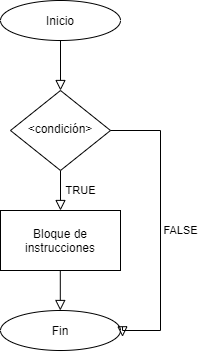
\includegraphics[width=0.5\textwidth,height=0.3\textheight]{../schemas/IF.png}
\caption{Ciclo IF}\label{id}
}
\end{figure}

para ver como funciona la función \emph{IF} podemos ejecutar las
siguientes lineas de código:

\begin{Shaded}
\begin{Highlighting}[]
\ControlFlowTok{if}\NormalTok{ (}\OtherTok{TRUE}\NormalTok{)\{}
  \KeywordTok{print}\NormalTok{(}\StringTok{"Es verdadero, ¡se ejecuta el bloque de código!"}\NormalTok{)}
\NormalTok{\}}
\end{Highlighting}
\end{Shaded}

\begin{verbatim}
## [1] "Es verdadero, ¡se ejecuta el bloque de código!"
\end{verbatim}

\begin{Shaded}
\begin{Highlighting}[]
\ControlFlowTok{if}\NormalTok{ (}\OtherTok{FALSE}\NormalTok{)\{}
  \KeywordTok{print}\NormalTok{(}\StringTok{"Es falso, ¡no se ejecuta la instrucción!"}\NormalTok{)}
\NormalTok{\}}
\end{Highlighting}
\end{Shaded}

Darle valores de TRUE o FALSE directamente a una funcion \emph{IF} es
poco común, lo que usualmente se hace es pasarle una expresión y esta al
ser evaluada retorna un TRUE o FALSE, como lo veremos en el siguiente
ejemplo, donde se generara un número aleatorio entre 0 y 1 y se
evaluara:

\begin{Shaded}
\begin{Highlighting}[]
\NormalTok{x <-}\StringTok{ }\KeywordTok{runif}\NormalTok{(}\DecValTok{1}\NormalTok{)}
\ControlFlowTok{if}\NormalTok{ (x }\OperatorTok{>}\StringTok{ }\FloatTok{0.5}\NormalTok{)\{}
  \KeywordTok{print}\NormalTok{(}\StringTok{"Este mensaje tiene un 50% de probabilidades de ser mostrado"}\NormalTok{)}
  \KeywordTok{print}\NormalTok{(x)}
\NormalTok{\}}
\end{Highlighting}
\end{Shaded}

\begin{verbatim}
## [1] "Este mensaje tiene un 50% de probabilidades de ser mostrado"
## [1] 0.5059046
\end{verbatim}

\hypertarget{else}{%
\subsection{ELSE}\label{else}}

El comando \emph{ELSE} es un complemento de la función \emph{IF} la cual
funciona de la siguiente manera, al evaluarse la función y dar un
resultado FALSE ejecutara un bloque de instrucciones, dicho
comportamiento lo podemos ver en el siguiente diagrama de flujo:

\begin{figure}
\hypertarget{id}{%
\centering
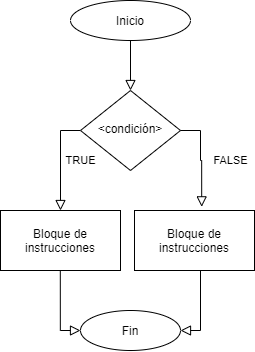
\includegraphics[width=0.5\textwidth,height=0.3\textheight]{../schemas/ELSE.png}
\caption{Ciclo ELSE}\label{id}
}
\end{figure}

El código después de un \emph{else} se ejecutara solo si el resultado de
la condición en \emph{if} es FALSE, podemos ver su estructura de la
siguiente manera:

\begin{verbatim}
if(<condicion>){
  Bloque de código
}else {
  Bloque de código
}
\end{verbatim}

Su ejecución seria de la siguiente manera:

\begin{Shaded}
\begin{Highlighting}[]
\NormalTok{x <-}\StringTok{ }\KeywordTok{runif}\NormalTok{(}\DecValTok{1}\NormalTok{)}
\ControlFlowTok{if}\NormalTok{ (x }\OperatorTok{>}\StringTok{ }\FloatTok{0.5}\NormalTok{)\{}
  \KeywordTok{cat}\NormalTok{(}\KeywordTok{c}\NormalTok{(x, }\StringTok{">"}\NormalTok{, }\StringTok{"0.5"}\NormalTok{))}
\NormalTok{\}}\ControlFlowTok{else}\NormalTok{\{}
  \KeywordTok{cat}\NormalTok{(}\KeywordTok{c}\NormalTok{(x, }\StringTok{"<"}\NormalTok{, }\StringTok{"0.5"}\NormalTok{))}
\NormalTok{\}}
\end{Highlighting}
\end{Shaded}

\begin{verbatim}
## 0.0601800105068833 < 0.5
\end{verbatim}

Las estructuras de control lógicas \emph{If} y \emph{If-else} permiten
tener mas estructuras de control dentro de si mismas dentro de los
bloques de código, a esto se le llama *anidación".

\hypertarget{for}{%
\subsection{FOR}\label{for}}

El bucle \emph{FOR} es una estructura iterativa que se ejecuta un número
de veces preestablecido, controlado por un contador. En el siguiente
Diagrama podemos ver el funcionamiento de este ciclo.

\begin{figure}
\hypertarget{id}{%
\centering
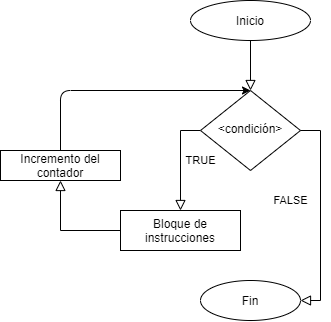
\includegraphics[width=0.5\textwidth,height=0.3\textheight]{../schemas/FOR.png}
\caption{Ciclo FOR}\label{id}
}
\end{figure}

Su estructura es la siguiente:

\begin{verbatim}
for(<contador> in <secuencia>){
  Bloque de código
}
\end{verbatim}

Algunos ejemplos serian los siguientes:

\begin{Shaded}
\begin{Highlighting}[]
\ControlFlowTok{for}\NormalTok{ (i }\ControlFlowTok{in} \DecValTok{1}\OperatorTok{:}\DecValTok{5}\NormalTok{)\{}
  \KeywordTok{print}\NormalTok{(i)}
\NormalTok{\}}
\end{Highlighting}
\end{Shaded}

\begin{verbatim}
## [1] 1
## [1] 2
## [1] 3
## [1] 4
## [1] 5
\end{verbatim}

\begin{Shaded}
\begin{Highlighting}[]
\NormalTok{suma <-}\StringTok{ }\DecValTok{0}
\ControlFlowTok{for}\NormalTok{ (i }\ControlFlowTok{in} \DecValTok{1}\OperatorTok{:}\DecValTok{5}\NormalTok{)\{}
\NormalTok{  suma <-}\StringTok{ }\NormalTok{suma }\OperatorTok{+}\StringTok{ }\NormalTok{i}
\NormalTok{\}}
\NormalTok{suma}
\end{Highlighting}
\end{Shaded}

\begin{verbatim}
## [1] 15
\end{verbatim}

\begin{Shaded}
\begin{Highlighting}[]
\CommentTok{# Vector aleatorio}
\NormalTok{x <-}\StringTok{ }\KeywordTok{sample}\NormalTok{(}\DecValTok{1}\OperatorTok{:}\DecValTok{50}\NormalTok{, }\DecValTok{100}\NormalTok{, }\DataTypeTok{replace=}\OtherTok{TRUE}\NormalTok{)}
\CommentTok{# inicializo la variable suma}
\NormalTok{suma <-}\StringTok{ }\DecValTok{0}
\CommentTok{# bucle for para calcular la media}
\ControlFlowTok{for}\NormalTok{ (i }\ControlFlowTok{in} \KeywordTok{seq_along}\NormalTok{(x))\{}
\NormalTok{  suma <-}\StringTok{ }\NormalTok{x[i] }\OperatorTok{+}\StringTok{ }\NormalTok{suma}
\NormalTok{  media <-}\StringTok{ }\NormalTok{suma}\OperatorTok{/}\KeywordTok{length}\NormalTok{(x)}
\NormalTok{\}}
\NormalTok{media}
\end{Highlighting}
\end{Shaded}

\begin{verbatim}
## [1] 24.94
\end{verbatim}

Con el ejemplo anterior podemos mejorarlo introduciendo un ciclo
condicional para ver un ejemplo de anidación.

\begin{Shaded}
\begin{Highlighting}[]
\CommentTok{# Vector aleatorio}
\NormalTok{x <-}\StringTok{ }\KeywordTok{sample}\NormalTok{(}\DecValTok{1}\OperatorTok{:}\DecValTok{50}\NormalTok{, }\DecValTok{100}\NormalTok{, }\DataTypeTok{replace=}\OtherTok{TRUE}\NormalTok{)}
\CommentTok{# inicializo la variable suma}
\NormalTok{suma <-}\StringTok{ }\DecValTok{0}
\CommentTok{# bucle for para calcular la media}
\ControlFlowTok{for}\NormalTok{ (i }\ControlFlowTok{in} \KeywordTok{seq_along}\NormalTok{(x))\{}
\NormalTok{  suma <-}\StringTok{ }\NormalTok{x[i] }\OperatorTok{+}\StringTok{ }\NormalTok{suma}
  \ControlFlowTok{if}\NormalTok{(i }\OperatorTok{==}\StringTok{ }\KeywordTok{length}\NormalTok{(x) )\{}
\NormalTok{    media <-}\StringTok{ }\NormalTok{suma}\OperatorTok{/}\KeywordTok{length}\NormalTok{(x)}
\NormalTok{  \}}
\NormalTok{\}}
\NormalTok{media}
\end{Highlighting}
\end{Shaded}

\begin{verbatim}
## [1] 25.63
\end{verbatim}

\hypertarget{while}{%
\subsection{WHILE}\label{while}}

El bucle \emph{while} se utiliza principalmente cuando no se sabe el
número de itraciones, este bucle se ejecutara mientras se cumple una
condición que se comprueba al principio de la instrucción. El diagrama
de flujo muestra su operación.

\begin{figure}
\hypertarget{id}{%
\centering
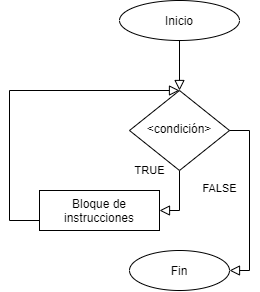
\includegraphics[width=0.5\textwidth,height=0.3\textheight]{../schemas/WHILE.png}
\caption{Ciclo WHILE}\label{id}
}
\end{figure}

Su estructura del bucle \emph{while} se muestra a continuación:

\begin{verbatim}
while(<condición>){
  Bloque de código
}
\end{verbatim}

Un ejemplo de ello serian los siguientes:

\begin{Shaded}
\begin{Highlighting}[]
\NormalTok{n <-}\StringTok{ }\DecValTok{1}
\ControlFlowTok{while}\NormalTok{ (n }\OperatorTok{<=}\StringTok{ }\DecValTok{5}\NormalTok{ )\{}
  \KeywordTok{print}\NormalTok{(n)}
\NormalTok{  n <-}\StringTok{ }\NormalTok{n }\OperatorTok{+}\DecValTok{1}
\NormalTok{\}}
\end{Highlighting}
\end{Shaded}

\begin{verbatim}
## [1] 1
## [1] 2
## [1] 3
## [1] 4
## [1] 5
\end{verbatim}

\begin{Shaded}
\begin{Highlighting}[]
\NormalTok{n <-}\StringTok{ }\DecValTok{1}
\ControlFlowTok{while}\NormalTok{ (n }\OperatorTok{<}\StringTok{ }\DecValTok{50}\NormalTok{ )\{}
\NormalTok{  n <-}\StringTok{ }\NormalTok{n }\OperatorTok{*}\DecValTok{2} \OperatorTok{+}\StringTok{ }\NormalTok{(n}\OperatorTok{+}\DecValTok{2}\NormalTok{)}
  \KeywordTok{print}\NormalTok{(n)}
\NormalTok{\}}
\end{Highlighting}
\end{Shaded}

\begin{verbatim}
## [1] 5
## [1] 17
## [1] 53
\end{verbatim}

\newpage
\singlespacing 
\end{document}